% Urban Heat Island — Łódź: research paper
% Build: pdflatex urban-heat-island-lodz.tex (twice). Figures in figures/ (made by pipeline/make_figures.py).

\documentclass[11pt,a4paper]{article}
\usepackage[utf8]{inputenc}
\usepackage[T1]{fontenc}
\usepackage{lmodern}
\usepackage{microtype}
\usepackage[margin=2.5cm]{geometry}
\usepackage{booktabs}
\usepackage{array}
\usepackage{parskip}
\usepackage{enumitem}
\usepackage{graphicx}
\usepackage{subcaption}
\usepackage{amsmath}
\usepackage{textcomp}
\usepackage[hidelinks]{hyperref}
\usepackage{url}
\usepackage{xurl}

\linespread{1.08}
\graphicspath{{figures/}}
\setlist{itemsep=2pt,topsep=4pt}

\newcommand{\repourl}{https://github.com/suadarzimanli/urban-heat-island-lodz}
\newcommand{\appurl}{https://suadarzimanli.github.io/urban-heat-island-lodz/}
\newcommand{\archivedoi}{; archived version: \href{https://doi.org/10.5281/zenodo.24438160}{doi:10.5281/zenodo.24438160}}

\title{Where Łódź Is Hot in Summer:\\ Vegetation, Built-up Land and Surface Heat from Twenty Clear Landsat Days}
\author{Suad Arzimanli\\[2pt]
        \small University of \L{}ód\'{z}, Faculty of Mathematics and Computer Science, Poland\\
        \small \texttt{suad.arzimanli@gmail.com}}
\date{}

\begin{document}
\maketitle

\begin{abstract}
Cities heat up unevenly, and planners need to know where and why. This paper maps summer surface heat across Łódź, Poland, and asks how much of its spatial pattern vegetation and built-up land explain, how stable that relationship is from day to day, and which places are hotter than those two factors predict. I used every June–August day from 2018 to 2025 on which at least 90\% of the city was cloud-free in Landsat 8 or 9 imagery --- twenty days --- and measured land surface temperature and vegetation (NDVI) from the same scenes, so that greenery and heat are observed at the same moment. Temperatures were expressed as anomalies from the city median of each day and averaged over a grid of 1,176 square 500~m cells; built-up share came from ESA WorldCover.

Surface heat is strongly clustered (Moran's $I = 0.76$): the 5th to 95th percentile of cells spans $-4.7$ to $+5.1$\,°C. Vegetation alone explains 90\% of its spatial variance ($R^2 = 0.896$; 0.894 when whole 2~km blocks are held out), with about 2\,°C less heat per 0.1 NDVI. Built-up share alone explains 70\%, and adds only one percentage point to vegetation because the two are strongly correlated ($r = -0.81$). The relationship holds on most single days (median $R^2 = 0.85$; 15 of 20 days above 0.75), at cell sizes of 250 to 1000~m, without edge cells, and with Sentinel-2 vegetation from other days. What vegetation does not explain is still spatially organised: the dense historic centre is cooler than its greenery predicts, while the airport and large industrial sites are hotter. An open, reproducible Python pipeline rebuilds every number from public satellite archives, and an interactive web map presents the results cell by cell.

\medskip
\noindent\textbf{Keywords:} urban heat island; land surface temperature; NDVI; Landsat; spatial autocorrelation; hot spots; Łódź.
\end{abstract}

%======================================================================
\section{Introduction}

Built-up areas run warmer than their surroundings: sealed surfaces store heat, vegetation that would cool through evaporation and shade is scarce, and buildings trap radiation \cite{oke1982}. Hot summers raise health risks and cooling demand, so cities increasingly plan green and blue infrastructure. Doing that well requires knowing where heat concentrates at neighbourhood scale and what explains it.

Satellite thermal imagery measures land surface temperature (LST) across a whole city at once \cite{voogt2003}. Many studies relate LST to vegetation indices such as NDVI and find a negative association whose strength varies with land-cover pattern, scale and season \cite{weng2004,zhou2011,peng2012}. Three practical questions are often left open: whether a relationship measured on one day holds on others, whether it survives the spatial dependence of neighbouring areas, and where a city departs from it.

Łódź is a useful case. A former textile-industry city with a dense nineteenth-century core, large housing estates, industrial zones, an airport and extensive forest in the north, it mixes nearly every urban surface type within its 293~km$^2$.

\subsection{Research questions}

\begin{description}[leftmargin=2.6em,style=nextline]
  \item[RQ1] How much of the spatial pattern of summer surface heat in Łódź do vegetation and built-up land explain, and how much does built-up land add to vegetation?
  \item[RQ2] Is the relationship stable across clear summer days, cell sizes and data sources?
  \item[RQ3] Which places are hotter or cooler than vegetation and built-up land predict, and where are the statistically significant hot and cold spots?
  \item[RQ4] Can the whole analysis be rebuilt from open data with open code and explored in a browser?
\end{description}

\subsection{Contributions}

\begin{enumerate}
  \item A reproducible pipeline that downloads Landsat 8/9, Sentinel-2 and ESA WorldCover data from a public archive, builds a metric 500~m grid and computes every statistic in this paper (\S\ref{sec:data}--\ref{sec:methods}).
  \item A multi-day analysis: twenty clear summer days from 2018 to 2025, with vegetation and temperature taken from the same scenes, and temperatures compared as daily anomalies.
  \item Robustness checks that respect spatial dependence: spatially blocked cross-validation, block bootstrap intervals, Moran's $I$ of residuals, three cell sizes, interior-only cells and an independent vegetation source (\S\ref{sec:results}).
  \item Maps of where the city is hotter or cooler than expected and of significant hot and cold spots, published in an interactive web map (\S\ref{sec:app}).
\end{enumerate}

%======================================================================
\section{Background}

\paragraph{Surface heat.} LST is the radiative temperature of the surfaces a satellite sees --- roofs, roads, canopy and soil --- not the air temperature people feel, although the two are linked, especially at night \cite{voogt2003}. The surface urban heat island is usually strongest on clear summer days around midday, when Landsat passes over central Europe at about 11:35 local time.

\paragraph{Vegetation and land cover.} NDVI, the normalised difference between near-infrared and red reflectance, measures green vegetation \cite{rouse1974}. Vegetated surfaces stay cooler through transpiration and shade, so NDVI and LST are negatively related \cite{weng2004}. The share of impervious or built-up land is an alternative explanation; because vegetation and sealing are two sides of the same land cover, the two are strongly correlated, and their configuration matters too \cite{zhou2011}.

\paragraph{Spatial data.} Neighbouring areas resemble each other, which inflates naive significance tests and in-sample fit. Moran's $I$ measures this dependence \cite{moran1950}; the local Getis–Ord $G_i^*$ statistic identifies clusters of high or low values \cite{ord1995}; and cross-validation that holds out whole spatial blocks gives an honest estimate of predictive skill \cite{roberts2017}. Results also depend on the size of the areal units, the modifiable areal unit problem \cite{openshaw1984}.

%======================================================================
\section{Study area and data}
\label{sec:data}

\paragraph{Boundary.} The administrative boundary of the city of Łódź (OpenStreetMap relation 2413295; 293.1~km$^2$), retrieved through the Nominatim service \cite{osm}.

\paragraph{Landsat 8 and 9.} Collection 2 Level-2 scenes from the Microsoft Planetary Computer archive \cite{planetary}, which requires no account. For every June–August day from 2018 to 2025 with less than 40\% scene cloud cover, the pipeline read the city's window and kept the scene if at least 90\% of the city was clear in the pixel quality band (no fill, cloud, cloud shadow, cirrus or snow). Twenty days qualified, from two satellite paths (Table~\ref{tab:dates} lists them with the city's median LST). Surface temperature is the official product, derived from the thermal band with atmospheric correction and emissivity from the ASTER Global Emissivity Dataset \cite{malakar2018,hulley2015}.

\paragraph{Sentinel-2.} Level-2A scenes from June to August 2023 with less than 10\% cloud; NDVI from bands 4 and 8 at 10~m, with clouds, shadows and snow removed using the scene classification, and the median of clear observations kept \cite{drusch2012}. It serves as an independent vegetation source.

\paragraph{ESA WorldCover 2021.} Land cover at 10~m \cite{zanaga2022}, used for the shares of built-up land, trees and water in each cell.

\begin{table}[htbp]
\centering
\small
\caption{The twenty clear summer days, with the city's median land surface temperature (°C) on each.}
\label{tab:dates}
\setlength{\tabcolsep}{5pt}
\begin{tabular}{lrlrlrlr}
\toprule
Day & LST & Day & LST & Day & LST & Day & LST \\
\midrule
4 Jul 2018 & 35.1 & 25 Jul 2020 & 31.1 & 9 Jul 2023 & 37.2 & 28 Aug 2024 & 33.4 \\
12 Aug 2018 & 24.9 & 17 Aug 2020 & 33.0 & 19 Aug 2023 & 34.4 & 29 Aug 2024 & 35.4 \\
12 Jun 2019 & 38.4 & 28 Jul 2021 & 35.6 & 9 Jun 2024 & 30.9 & 21 Jun 2025 & 32.9 \\
24 Aug 2019 & 31.1 & 5 Jun 2022 & 29.6 & 26 Jun 2024 & 37.5 & 15 Aug 2025 & 35.7 \\
31 Aug 2019 & 35.6 & 8 Jun 2023 & 35.8 & 13 Aug 2024 & 31.6 & 16 Aug 2025 & 34.3 \\
\bottomrule
\end{tabular}
\end{table}

%======================================================================
\section{Methods}
\label{sec:methods}

\subsection{Common grid}

All data were resampled onto one analysis grid of 10~m pixels in UTM zone 34N (EPSG:32634), which covers the city with a 1.5~km margin. Landsat's 30~m pixels map onto 3$\times$3 blocks of the grid. Square cells of 250, 500 and 1000~m contain whole pixels; a cell is kept when at least half of its area lies inside the city boundary, giving 1,176 cells of 500~m. Water pixels are excluded from all temperature and vegetation averages, and cells that are more than half water are dropped.

\subsection{Surface temperature and its gaps}

The Landsat surface-temperature product is empty over 3.5\% of the city on every day, although these pixels are clear: the ASTER emissivity input is missing there, so the product leaves them blank. To keep these areas, temperature was recomputed from the product's own intermediate layers --- thermal radiance $L_\text{TOA}$, upwelling and downwelling radiance $L_\uparrow, L_\downarrow$ and atmospheric transmittance $\tau$ --- with an emissivity $\varepsilon$ estimated from NDVI \cite{sobrino2004}:
\begin{equation}
L_\text{s} = \frac{L_\text{TOA} - L_\uparrow - \tau (1 - \varepsilon) L_\downarrow}{\tau\, \varepsilon}, \qquad
T = \frac{K_2}{\ln\!\left(K_1 / L_\text{s} + 1\right)},
\end{equation}
where $K_1, K_2$ are the thermal band's calibration constants from the scene metadata. The NDVI–emissivity relationship is learned on each scene from its valid pixels (median product emissivity in NDVI bins of 0.02). Recomputing valid pixels with the product's own emissivity reproduces the official temperatures to within 0.2~K; with the NDVI-based emissivity, the error is 0.51--0.60~K (RMSE after removing a scene-wide offset of about 0.1~K). Filled pixels are flagged, and the analysis is repeated without them.

\subsection{Anomalies, vegetation and land cover}

Clear days differ in weather: the city's median LST ranges from 24.9 to 38.4\,°C. Each cell's mean LST on a day was therefore expressed as an \emph{anomaly}, its difference from the median of all cells that day. A cell is valid on a day when at least 70\% of its land pixels are clear, and enters the multi-day analysis when it is valid on at least 75\% of the days; all 1,176 cells meet this. The \emph{surface heat} of a cell is its mean anomaly over the days on which it is valid. NDVI was computed from the red and near-infrared bands of the same Landsat scenes, so that vegetation and temperature refer to the same moment; it was averaged in the same way. Built-up, tree and water shares come from WorldCover.

\subsection{Statistics}

Surface heat was regressed on NDVI, on built-up share, and on both, by ordinary least squares. Because neighbouring cells are dependent, three safeguards were used: (i) spatially blocked five-fold cross-validation, holding out whole 2~km blocks; (ii) 95\% intervals for coefficients from a bootstrap that resamples whole blocks (999 replicates); and (iii) Moran's $I$ of the model residuals with rook contiguity and a permutation test. Local hot and cold spots were identified with the Getis–Ord $G_i^*$ statistic over each cell and its eight neighbours, with $p$-values controlled at a 5\% false-discovery rate \cite{benjamini1995}. The same regressions were repeated for each day, for 250 and 1000~m cells, for interior cells only, without gap-filled cells, and with Sentinel-2 NDVI.

%======================================================================
\section{Results}
\label{sec:results}

\subsection{The pattern of surface heat}

Figure~\ref{fig:maps} shows the mean summer surface heat at 30~m alongside vegetation and built-up land. The hottest areas are the city centre, large industrial and commercial sites in the north-west, east and south, and the airport in the south-west; the coolest are the Łagiewniki forest in the north, parks, and the green outskirts. Across 500~m cells the anomaly ranges from $-7.7$ to $+10.5$\,°C (5th to 95th percentile $-4.7$ to $+5.1$\,°C). The pattern is strongly clustered: Moran's $I = 0.76$ ($p = 0.001$).

\begin{figure}[htbp]
\centering
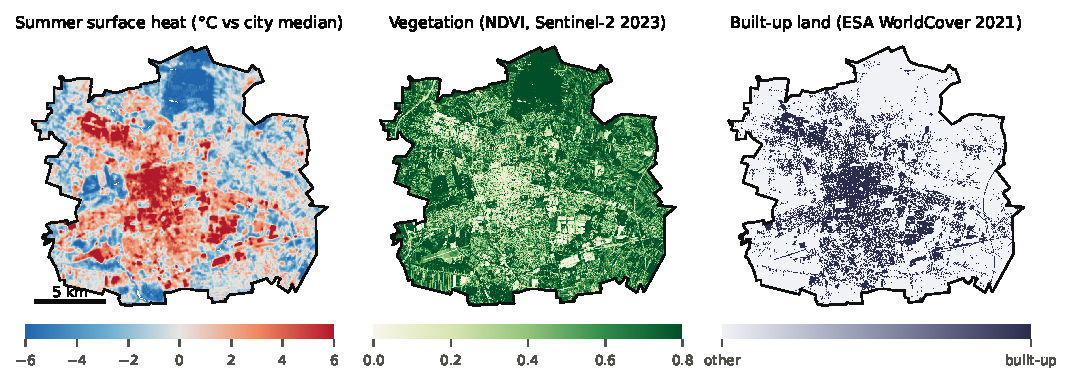
\includegraphics[width=\linewidth]{fig-maps.pdf}
\caption{Mean summer surface heat over twenty clear days (Landsat, 30~m; temperature minus the city median of each day), vegetation (Sentinel-2 NDVI, summer 2023) and built-up land (ESA WorldCover 2021). Water is left blank.}
\label{fig:maps}
\end{figure}

\subsection{How much vegetation and built-up land explain (RQ1)}

Table~\ref{tab:models} and Figure~\ref{fig:scatter} give the results. Vegetation alone explains 90\% of the spatial variance of surface heat ($R^2 = 0.896$), and almost all of it carries over to held-out areas (blocked cross-validated $R^2 = 0.894$). The slope is $-20.5$\,°C per NDVI unit, about 2\,°C less heat for each 0.1 of NDVI (95\% block-bootstrap interval $-21.4$ to $-19.4$). Built-up share alone explains 70\%. Adding built-up share to vegetation raises $R^2$ by just over one percentage point, because the two measure largely the same thing ($r = -0.81$); in the joint model, each extra 10 percentage points of built-up land adds 0.2\,°C (interval 0.12 to 0.29\,°C). Water share and distance from the centre add nothing further.

\begin{table}[htbp]
\centering
\small
\caption{Regressions of summer surface heat on 1,176 cells of 500~m. Blocked CV: five-fold cross-validation holding out whole 2~km blocks. Moran's $I$ of the surface heat itself is 0.76.}
\label{tab:models}
\begin{tabular}{lrrrl}
\toprule
Explanatory variables & $R^2$ & Blocked-CV $R^2$ & Residual Moran's $I$ & Coefficients \\
\midrule
Vegetation (NDVI) & 0.896 & 0.894 & 0.54 & $-20.5$ per NDVI unit \\
Built-up share & 0.699 & 0.691 & 0.66 & $+8.9$ per unit share \\
Vegetation + built-up share & 0.909 & 0.905 & 0.48 & $-17.0$, $+2.1$ \\
+ water, distance to centre & 0.910 & 0.905 & 0.48 & --- \\
\bottomrule
\end{tabular}
\end{table}

\begin{figure}[htbp]
\centering
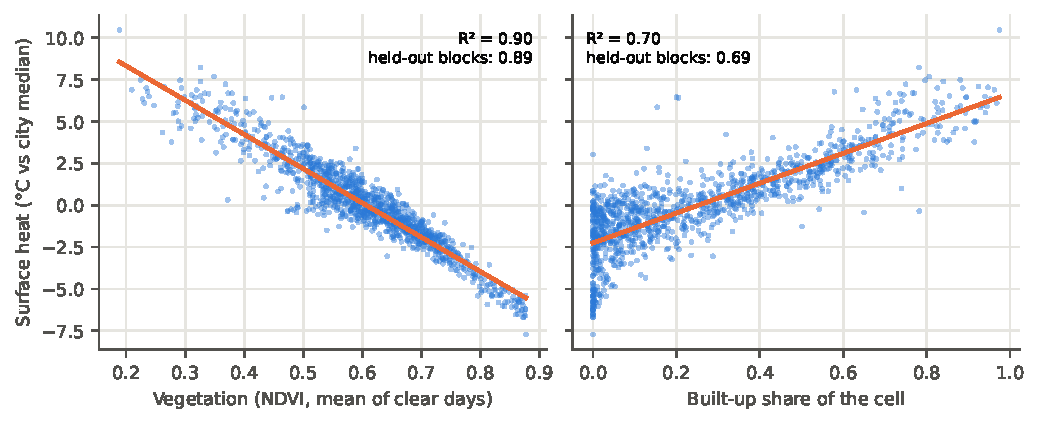
\includegraphics[width=\linewidth]{fig-scatter.pdf}
\caption{Summer surface heat of each 500~m cell against vegetation and against built-up share, with least-squares lines.}
\label{fig:scatter}
\end{figure}

\subsection{Stability across days, scales and data (RQ2)}

The relationship holds on most single days (Figure~\ref{fig:dates}). Vegetation alone explains a median of 85\% of the spatial variance per day (range 39--91\%), and more than 75\% on 15 of 20 days; the slope ranges from $-1.5$ to $-2.5$\,°C per 0.1 NDVI. The weakest days --- 28 July 2021, 12 August 2018, 17 August 2020 and 4 July 2018 --- include the coolest day in the set (median LST 24.9\,°C) and the two days with the most cloud-masked area (5--7\% of the city). Built-up share usually adds little to vegetation on a single day (median 0.9 percentage points), but on some days it adds more, up to 15 points on 25 July 2020. The steepness of the slope is unrelated to how hot the day was ($r = 0.17$ between slope and median LST).

\begin{figure}[htbp]
\centering
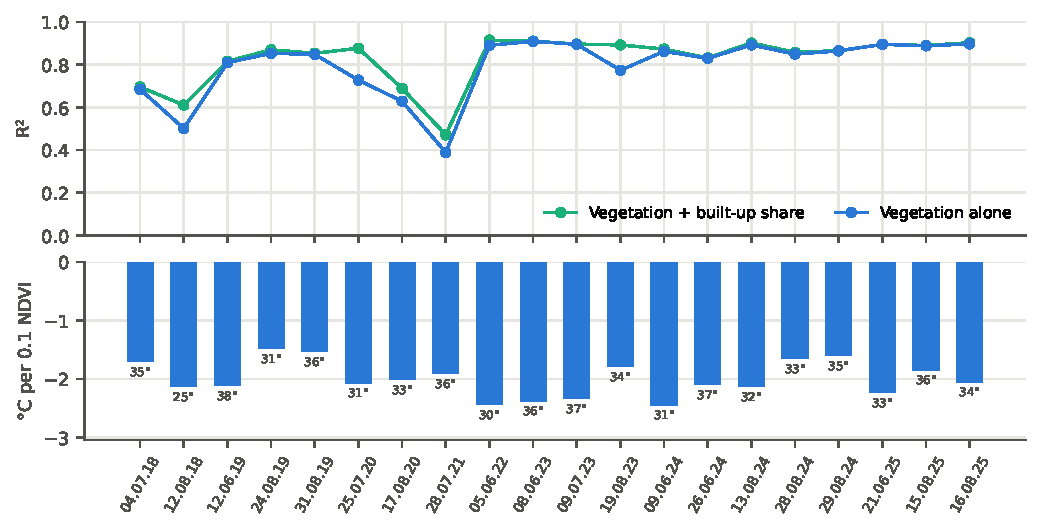
\includegraphics[width=\linewidth]{fig-dates.pdf}
\caption{Each clear day separately. Top: share of the spatial variance of surface heat explained by vegetation alone and by vegetation plus built-up share. Bottom: temperature change per 0.1 NDVI, with the city's median LST that day.}
\label{fig:dates}
\end{figure}

The result does not depend on the analysis choices (Table~\ref{tab:robust}). Larger cells average out small-scale noise and raise $R^2$ slightly, as expected from the modifiable areal unit problem; even at 250~m, vegetation explains 86\%. Edge cells, gap-filled temperatures and the choice of vegetation sensor make no material difference: Sentinel-2 NDVI from other days correlates at 0.99 with the Landsat NDVI and explains 88\% of the variance on 8 June 2023.

\begin{table}[htbp]
\centering
\small
\caption{Robustness: share of variance of summer surface heat explained ($R^2$).}
\label{tab:robust}
\begin{tabular}{lrrr}
\toprule
Variant & Cells & Vegetation & Vegetation + built-up \\
\midrule
500~m cells (main) & 1,176 & 0.896 & 0.909 \\
250~m cells & 4,695 & 0.860 & 0.873 \\
1000~m cells & 293 & 0.914 & 0.931 \\
Interior cells only (wholly inside the city) & 1,060 & 0.898 & 0.910 \\
Without cells containing gap-filled temperature & 1,086 & 0.901 & 0.911 \\
8 June 2023, Landsat NDVI & 1,176 & 0.909 & --- \\
8 June 2023, Sentinel-2 summer NDVI & 1,176 & 0.884 & --- \\
\bottomrule
\end{tabular}
\end{table}

\subsection{Where Łódź departs from the expectation (RQ3)}

The residuals of the joint model are themselves clustered (Moran's $I = 0.48$), so what vegetation and built-up land do not explain is organised in space rather than random (Figure~\ref{fig:residuals}, left). Ninety-six cells are more than 1\,°C hotter than expected and 111 more than 1\,°C cooler. The dense historic centre is cooler than its scarce vegetation predicts: the 50 cells within 2~km of the centre are 3.6\,°C hotter than the city median on average but 0.6\,°C cooler than expected, consistent with shading in narrow streets between tall buildings and with materials that heat more slowly than flat roofs and open paving. Hotter-than-expected cells concentrate on the airport, where dry grass and runways heat strongly despite moderate NDVI, and on large industrial and commercial sites with extensive flat roofs and paved yards.

The $G_i^*$ statistic identifies 181 hot-spot and 120 cold-spot cells at a 5\% false-discovery rate (Figure~\ref{fig:residuals}, right). The hot spots form a continuous belt from the centre to the north-west and south-east; 176 of the 181 have below-median vegetation. The cold spots are the northern forest, a large park complex in the west and green areas at the southern edge.

\begin{figure}[htbp]
\centering
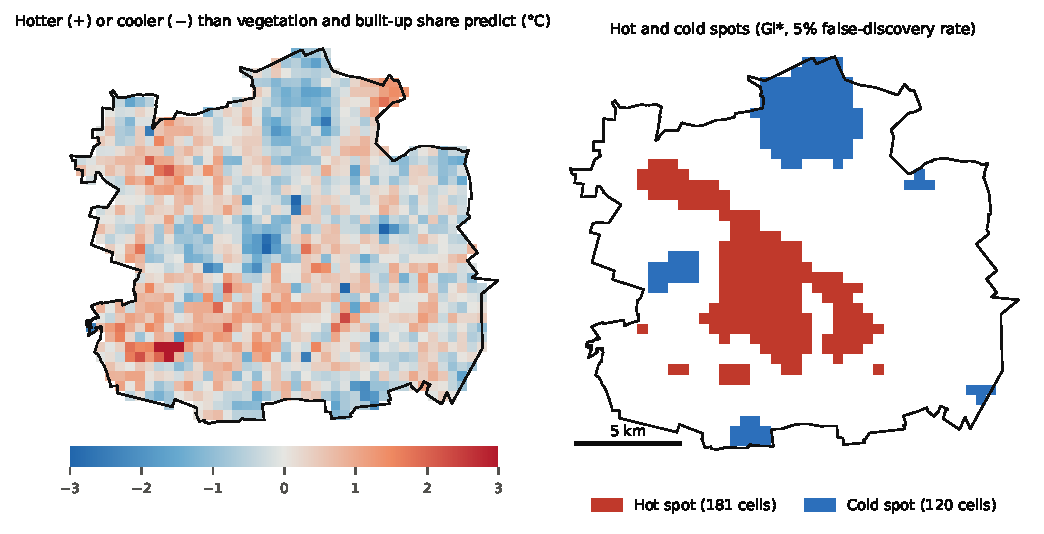
\includegraphics[width=\linewidth]{fig-residuals.pdf}
\caption{Left: how much hotter (+) or cooler ($-$) each cell is than vegetation and built-up share predict. Right: significant hot and cold spots of summer surface heat (Getis–Ord $G_i^*$, 5\% false-discovery rate).}
\label{fig:residuals}
\end{figure}

%======================================================================
\section{The web map (RQ4)}
\label{sec:app}

The results are published as a static web application (Leaflet and Chart.js) that reads the pipeline's outputs and runs without a server (Figure~\ref{fig:app}). Users choose what the map shows --- surface heat, vegetation, built-up share, hotter or cooler than expected, or hot and cold spots --- and whether to show the satellite pixels (the default: 30~m Landsat surface heat and vegetation, 10~m built-up land) or the 500~m grid, whose cells are the averages of those pixels; residuals and hot spots exist only for cells. A date selector shows any of the twenty days or their mean. Clicking a cell shows its values, the expected heat from its vegetation and built-up share, and its anomaly on each day; a scatter plot of all cells is linked to the map in both directions. Legends state values in °C or NDVI. The grid cells, their values on each day and the boundary can be downloaded as CSV and GeoJSON.

\begin{figure}[htbp]
\centering
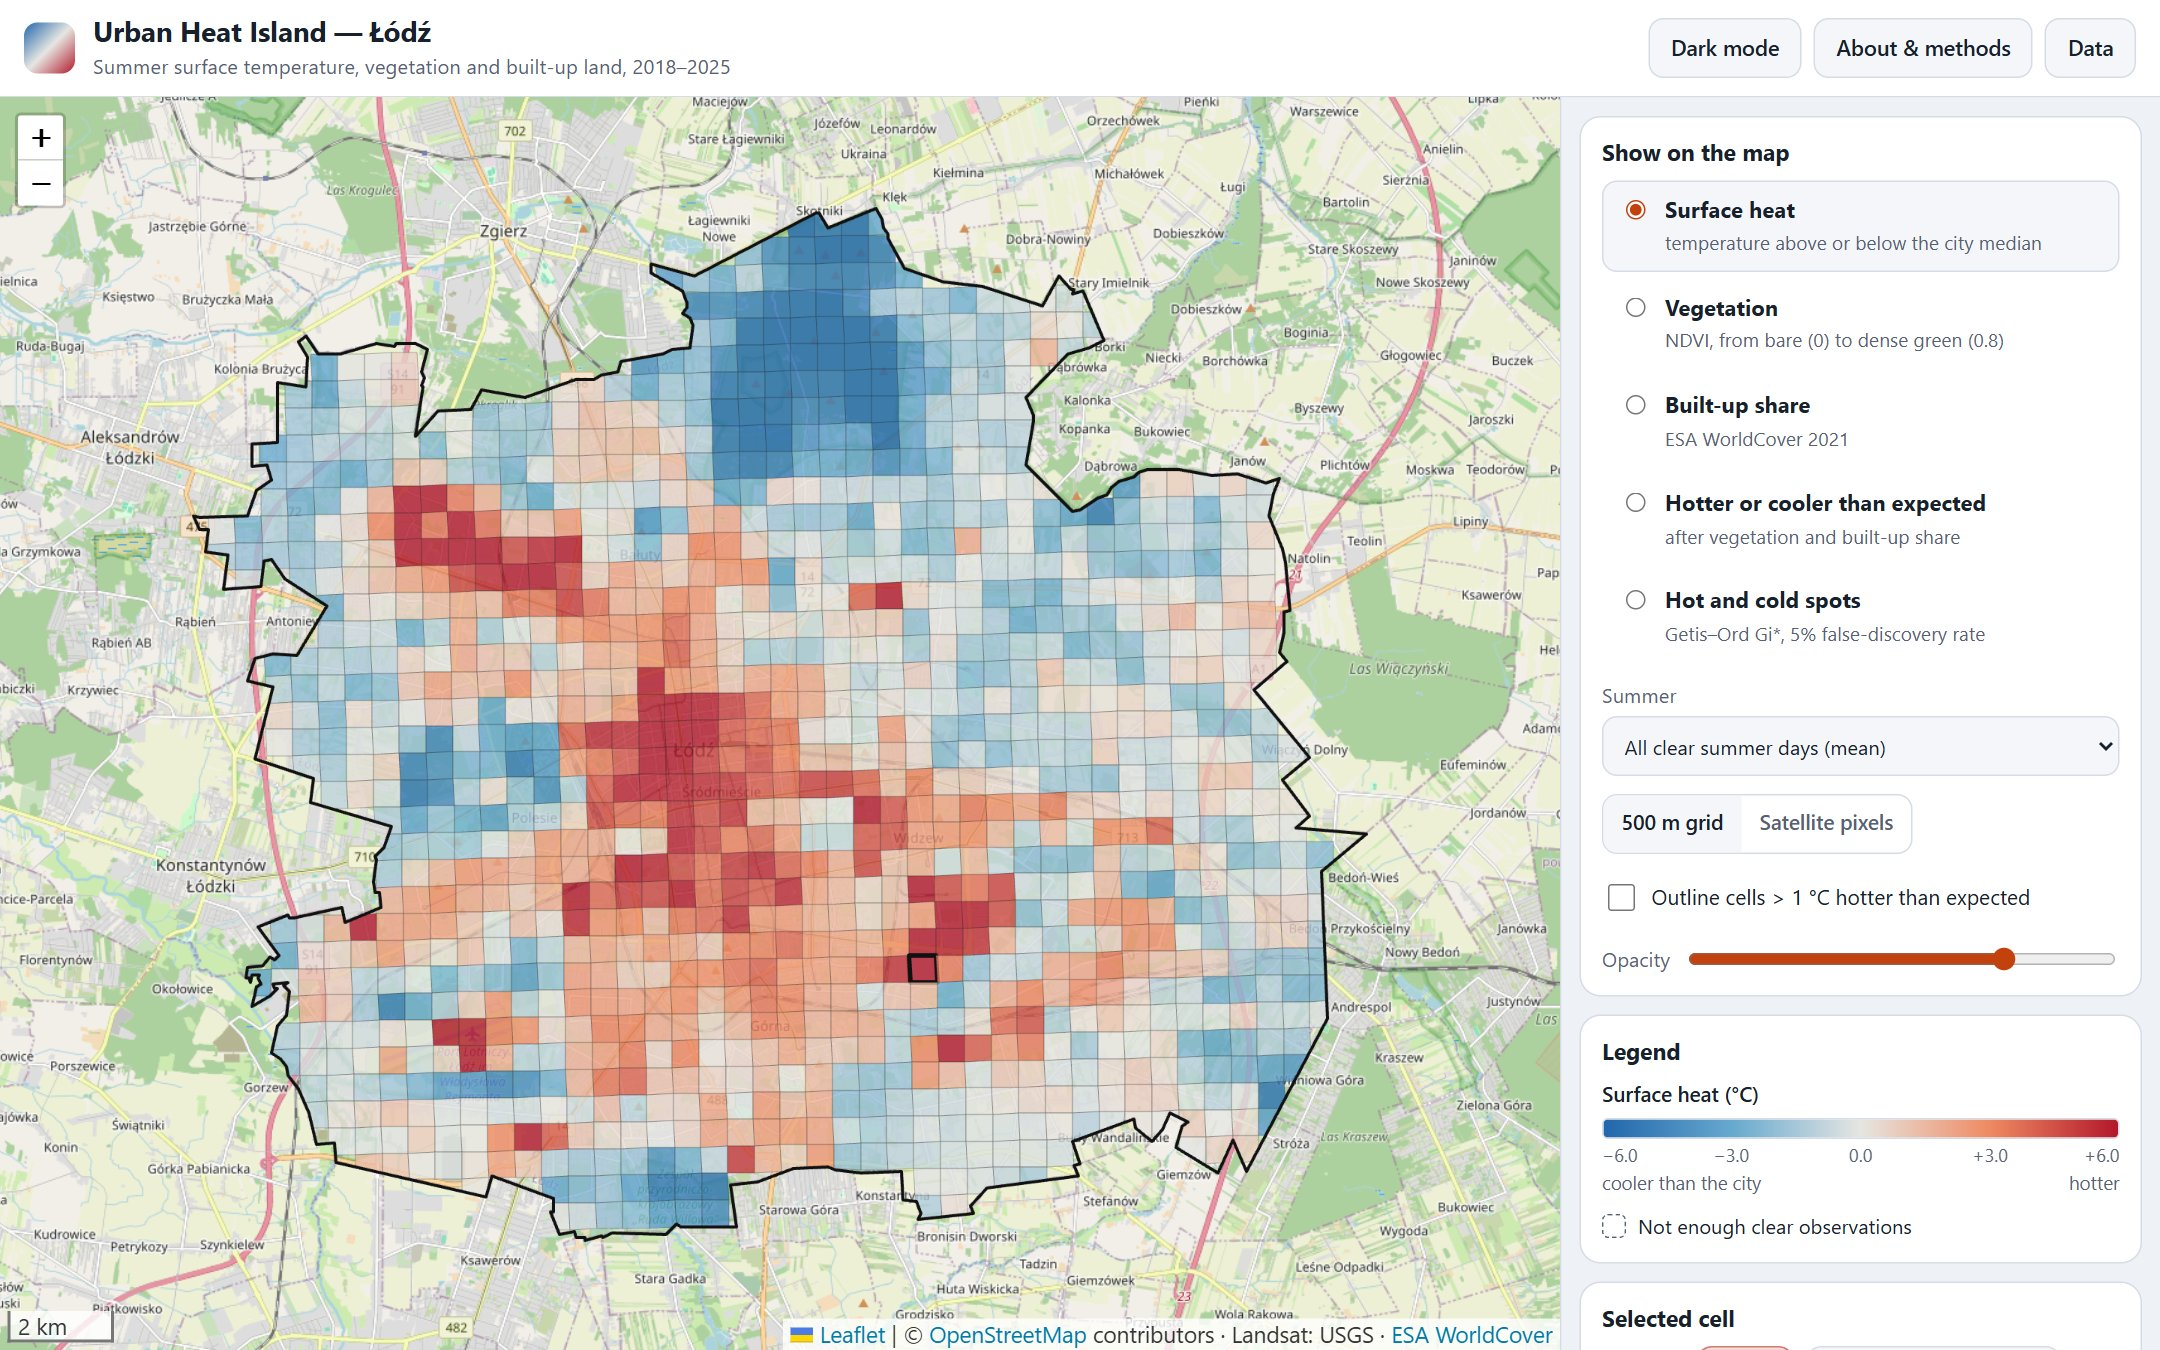
\includegraphics[width=\linewidth]{app-overview.jpg}
\caption{The web map: summer surface heat on the 500~m grid, with controls, legend and the hottest cell selected.}
\label{fig:app}
\end{figure}

\begin{figure}[htbp]
\centering
\begin{subfigure}{0.49\linewidth}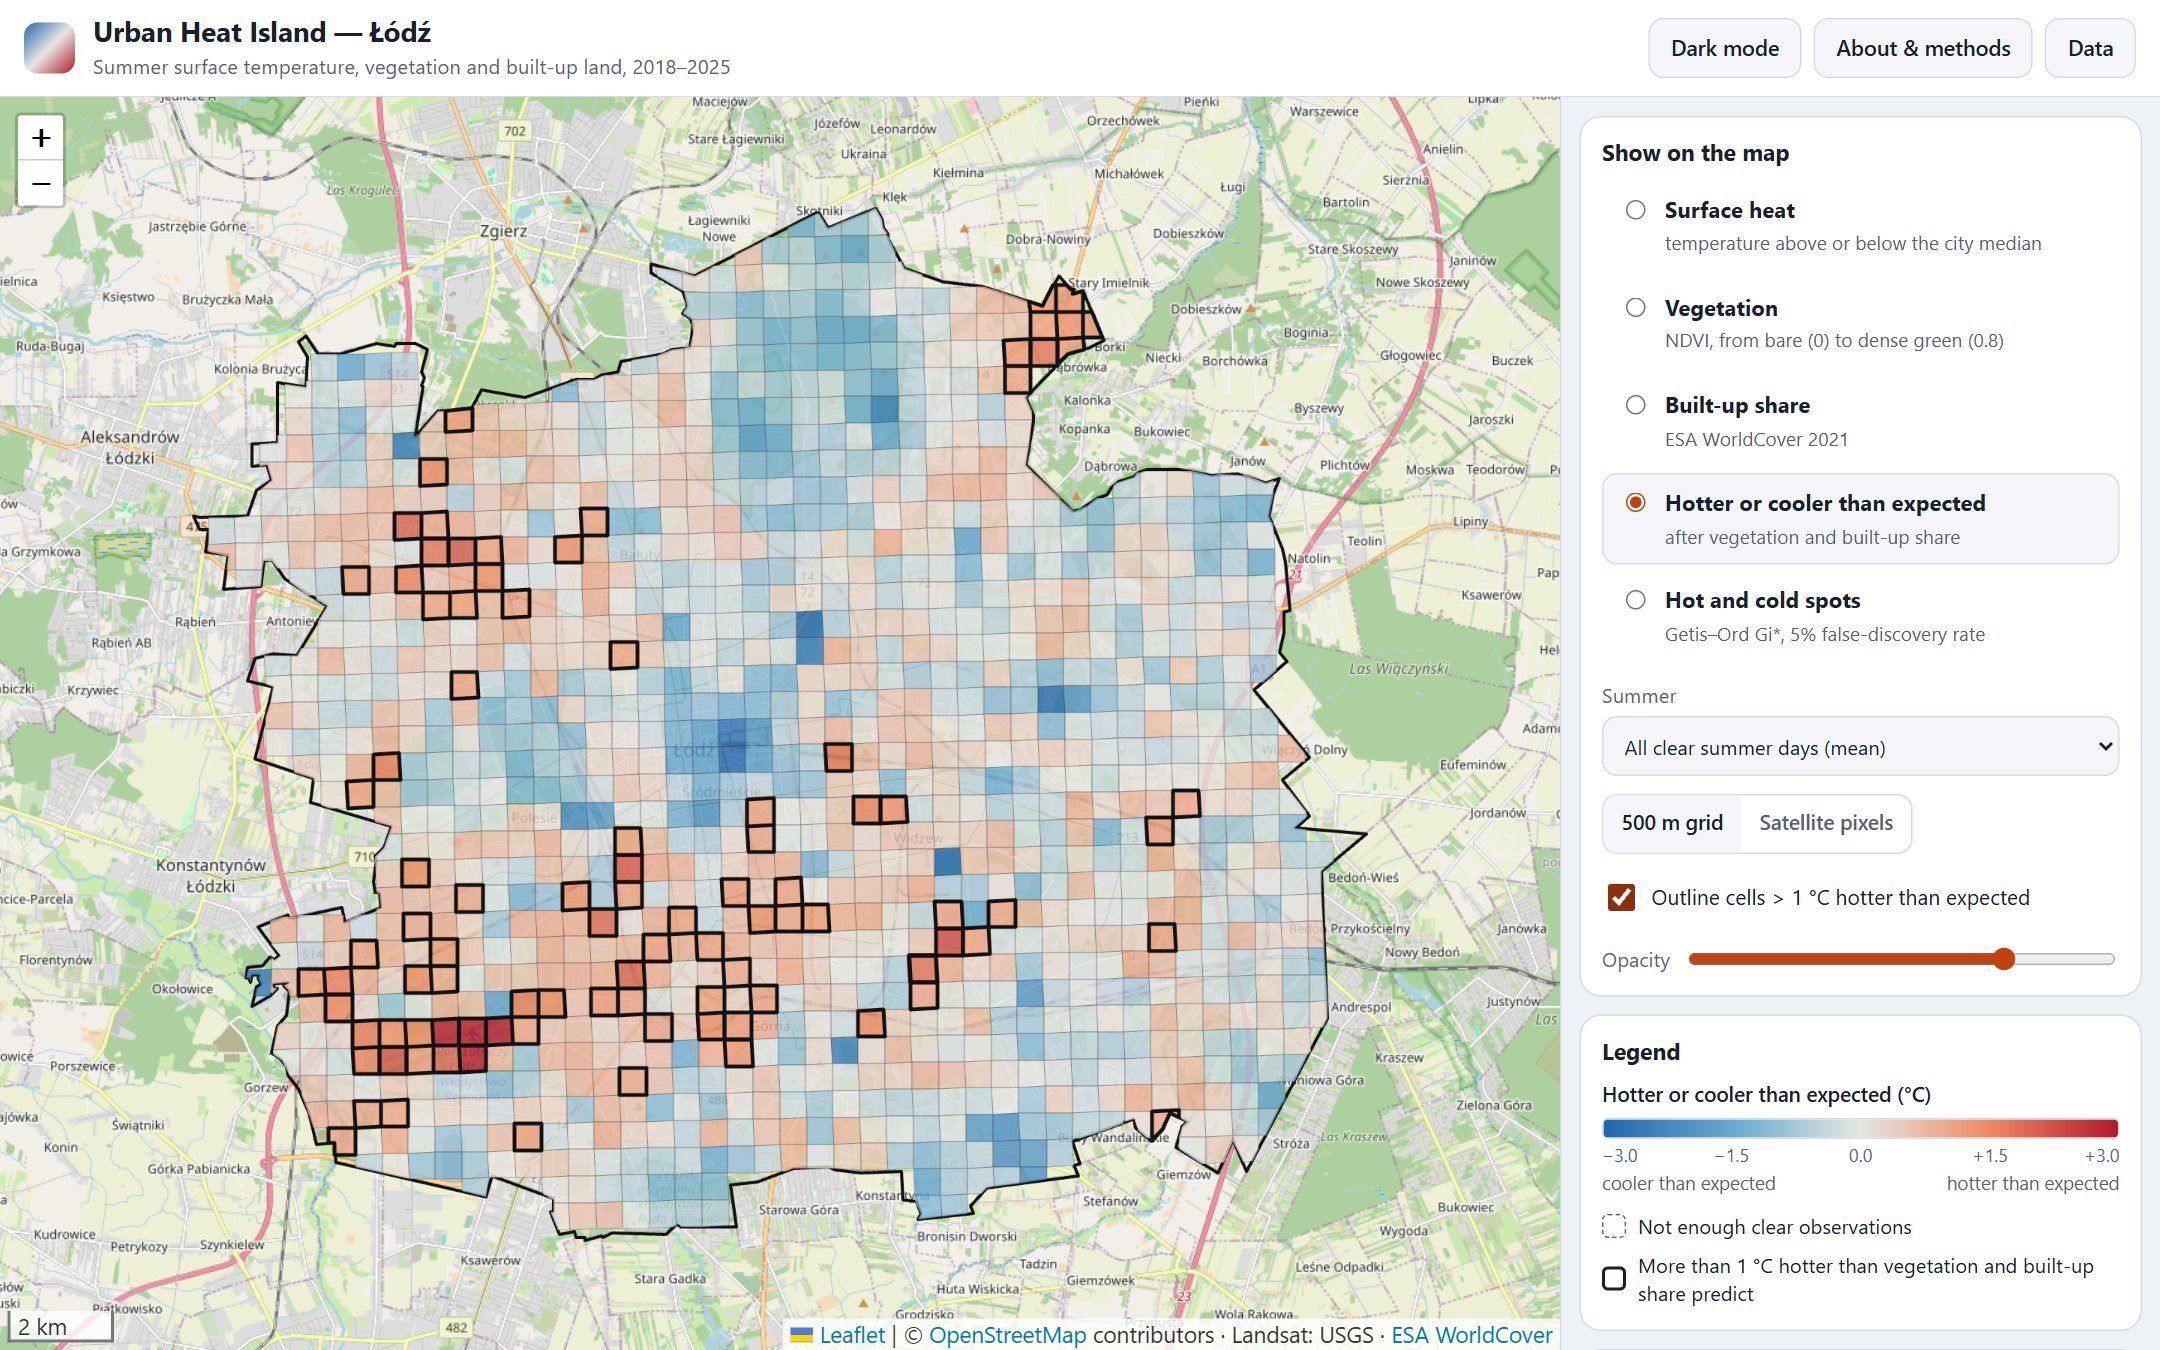
\includegraphics[width=\linewidth]{app-residual.jpg}\caption{Hotter or cooler than expected, with cells more than 1\,°C hotter outlined}\end{subfigure}\hfill
\begin{subfigure}{0.49\linewidth}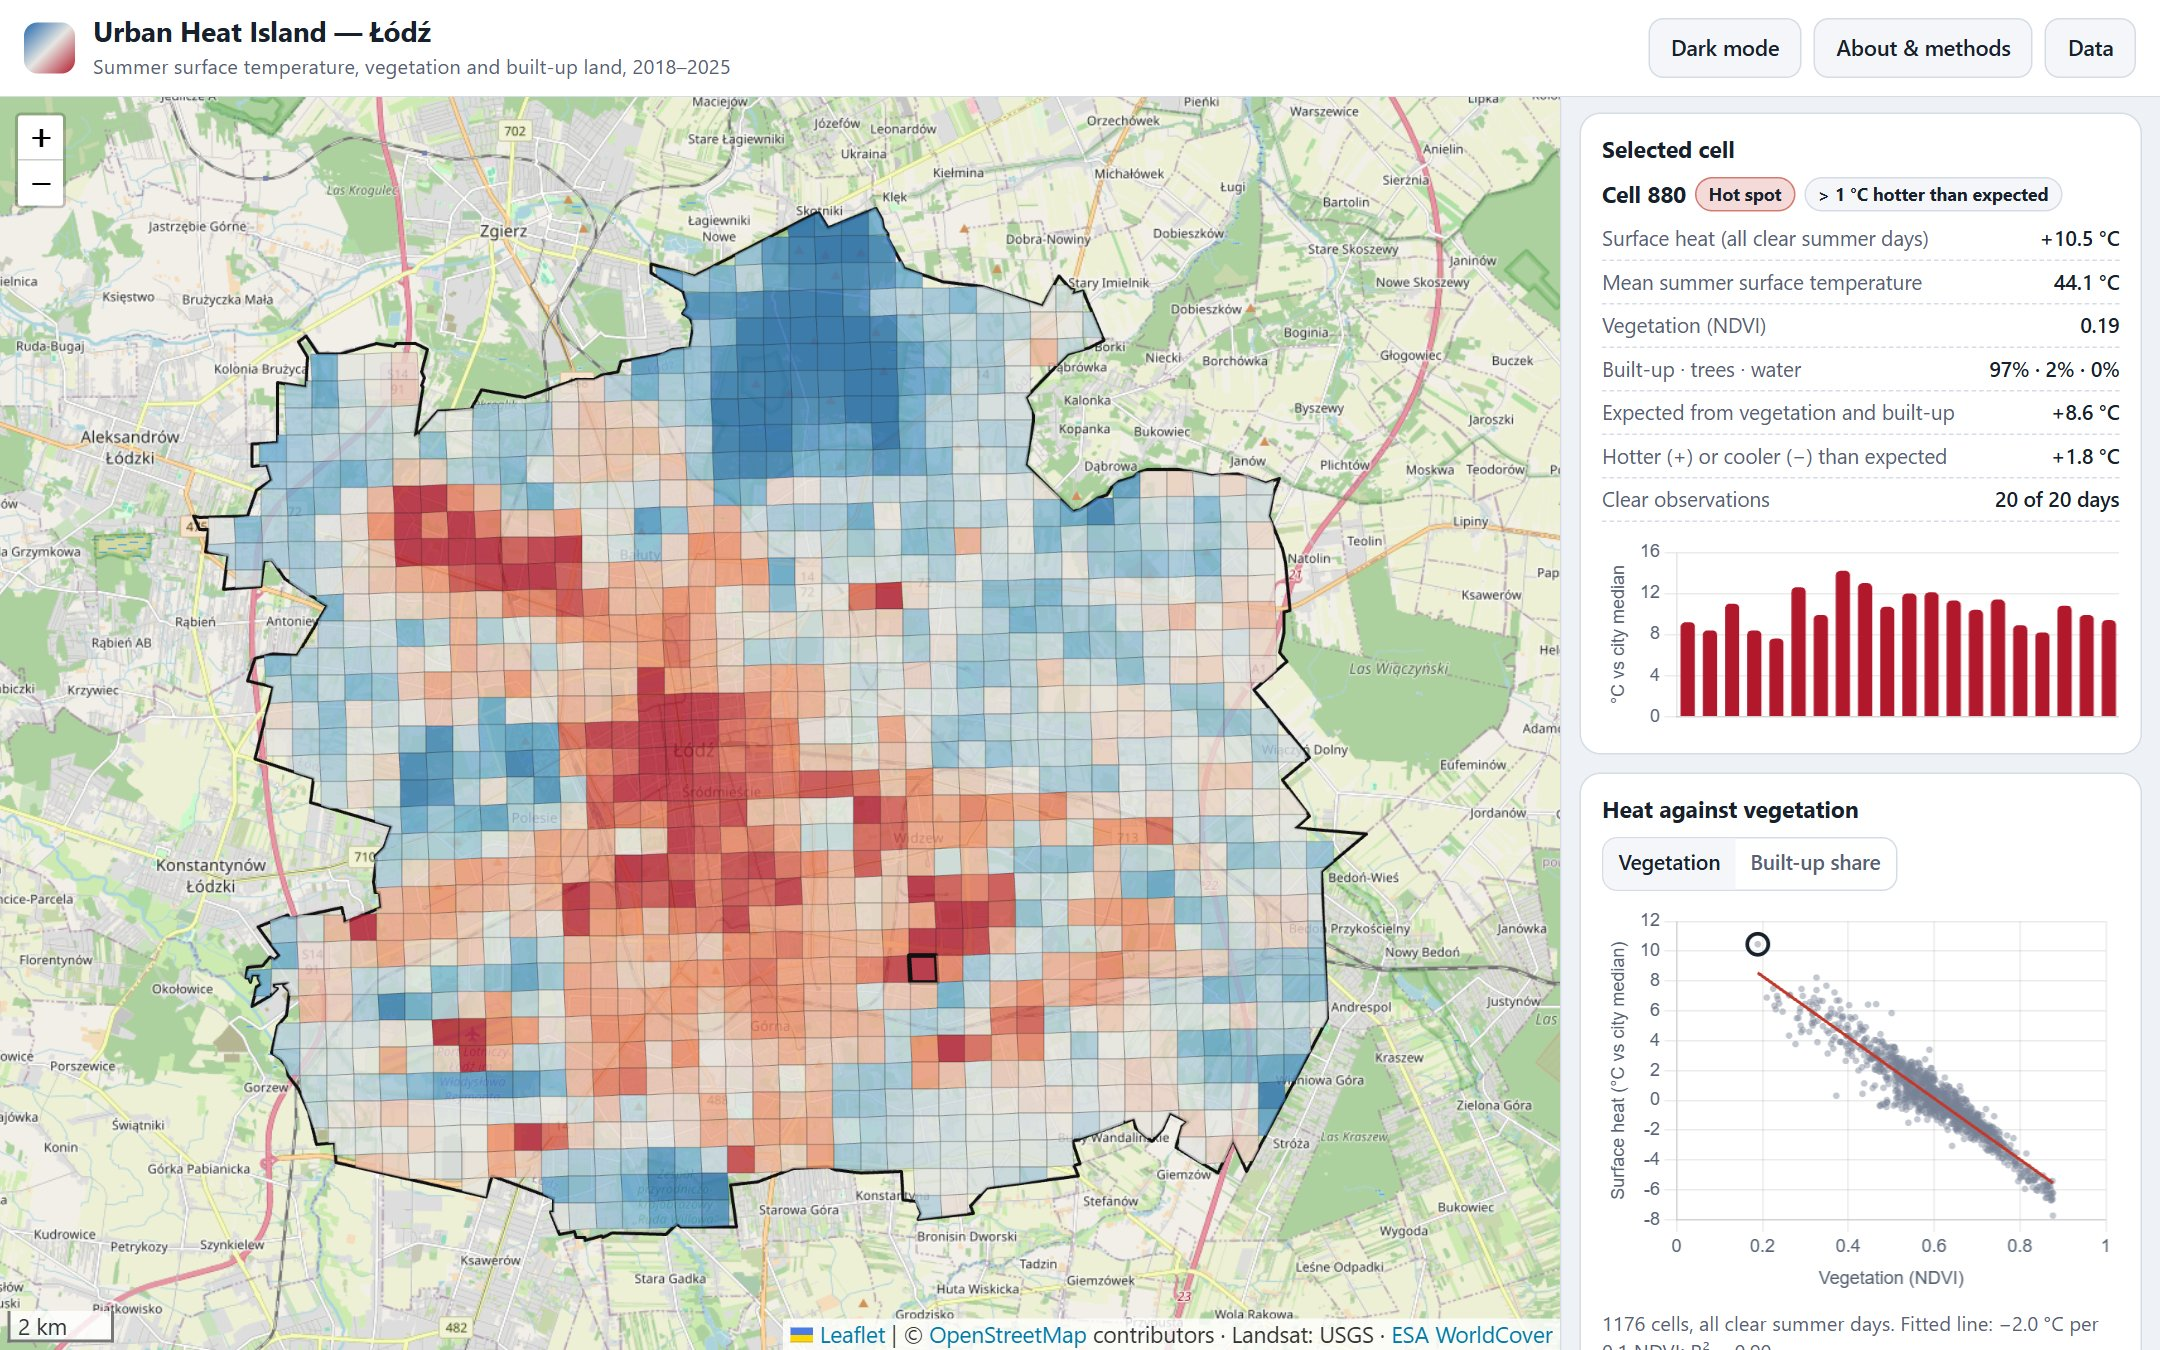
\includegraphics[width=\linewidth]{app-panel.jpg}\caption{Selected cell: its values, its anomaly on each day, and the linked scatter plot}\end{subfigure}
\caption{Two further views of the web map.}
\label{fig:app2}
\end{figure}

The interface follows the analysis: colour scales are diverging for anomalies and residuals (blue, neutral grey, red) and sequential for vegetation and built-up share; cells with too few clear observations are marked rather than coloured; the panel and the map stack on phones, with touch targets of at least 44\,px (Figure~\ref{fig:phone}). Fifteen Python unit tests cover the temperature conversion and gap filling, cloud masking, the grid, zonal statistics, Moran's $I$, $G_i^*$, the false-discovery rate and blocked cross-validation; six JavaScript tests check the colour scales, formatting and that the web data match the analysis.

\begin{figure}[htbp]
\centering
\begin{subfigure}{0.31\linewidth}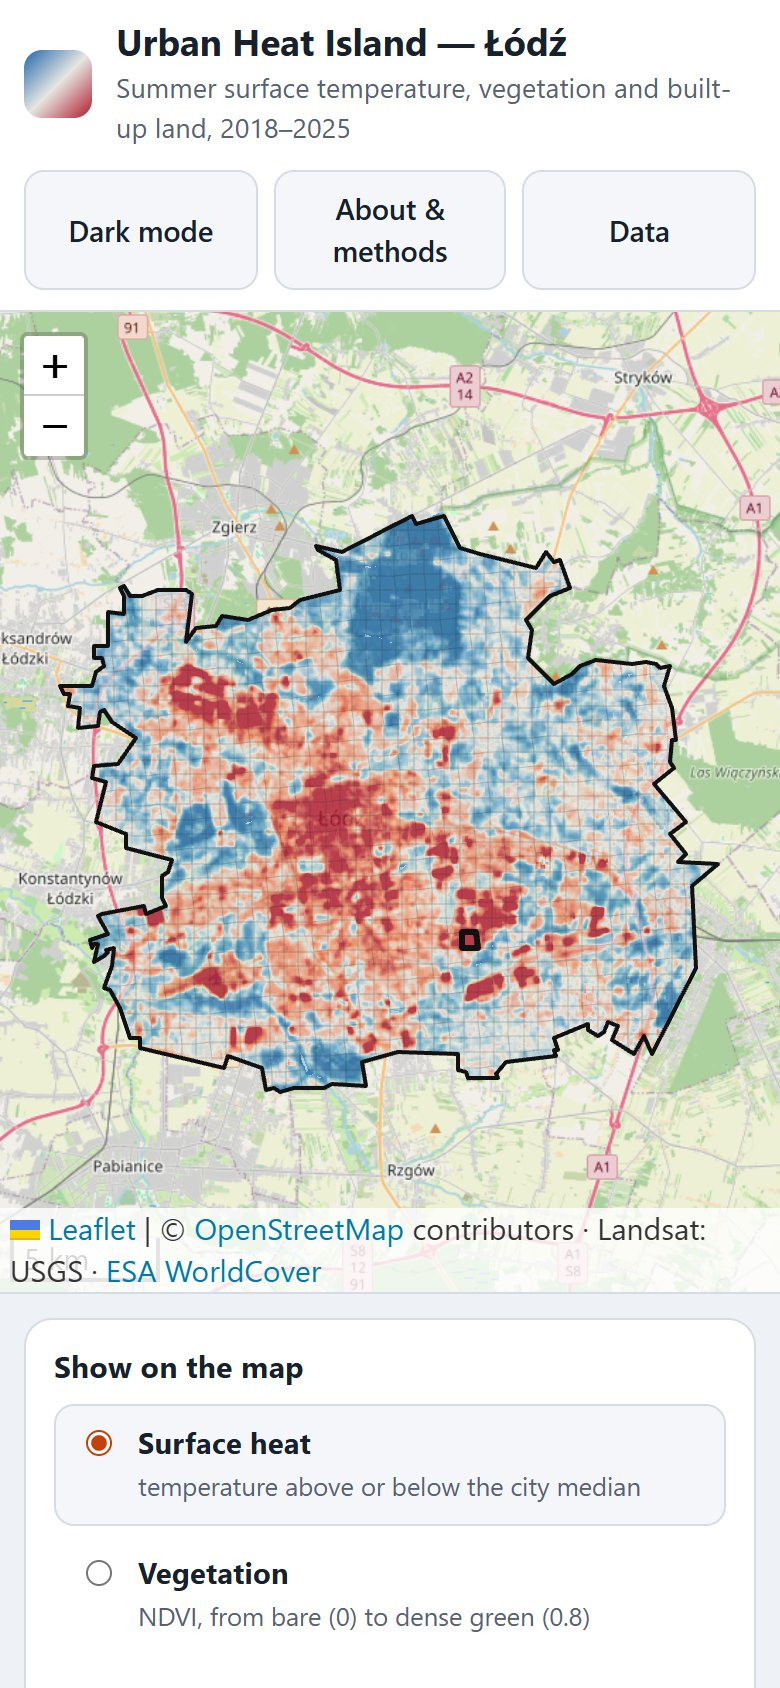
\includegraphics[width=\linewidth]{phone-map.jpg}\caption{Map}\end{subfigure}\hfill
\begin{subfigure}{0.31\linewidth}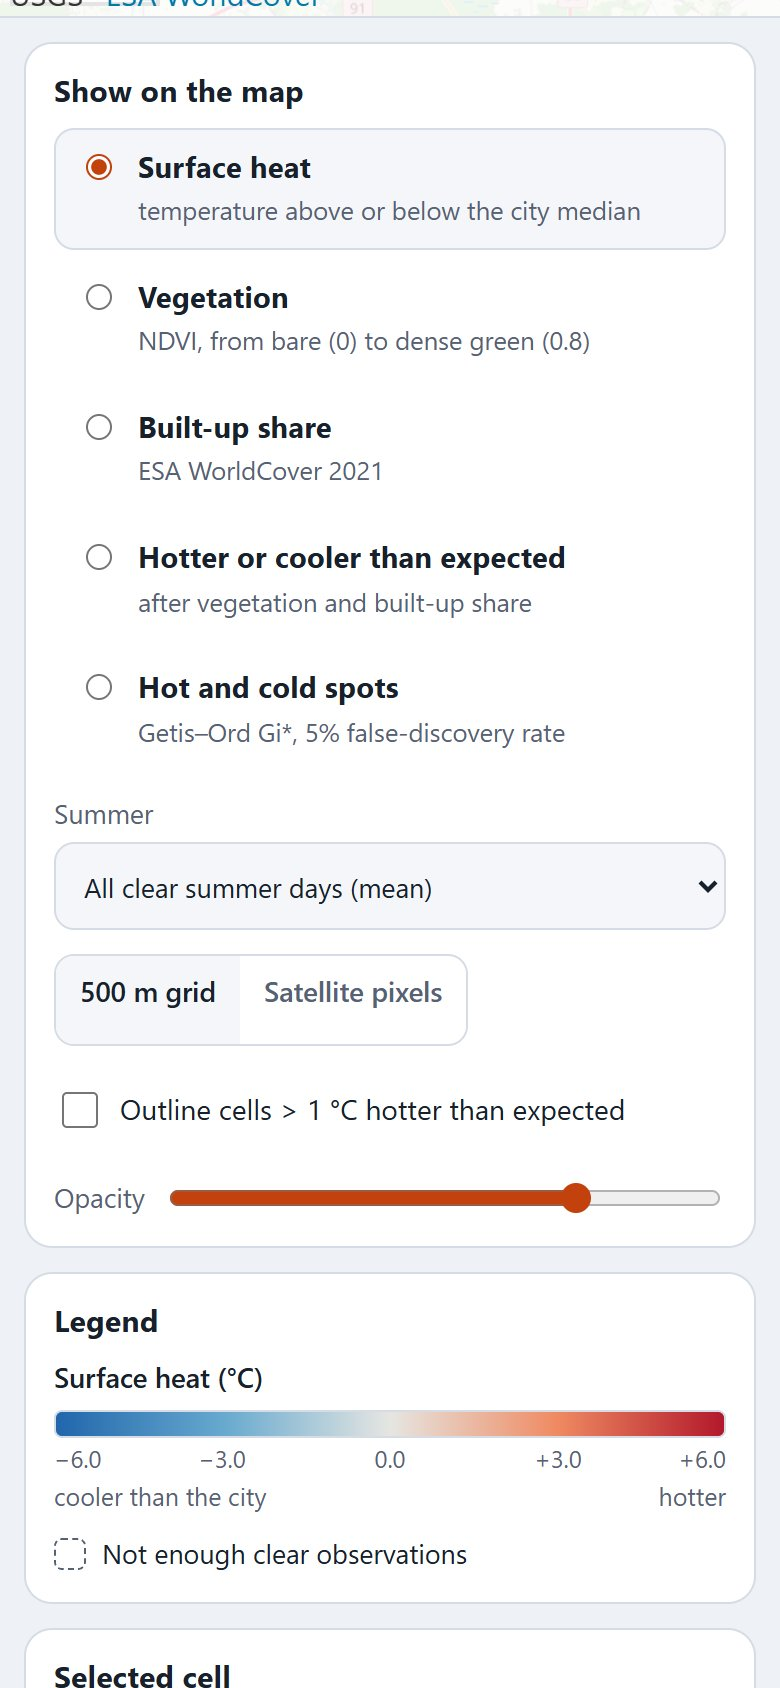
\includegraphics[width=\linewidth]{phone-controls.jpg}\caption{Controls and legend}\end{subfigure}\hfill
\begin{subfigure}{0.31\linewidth}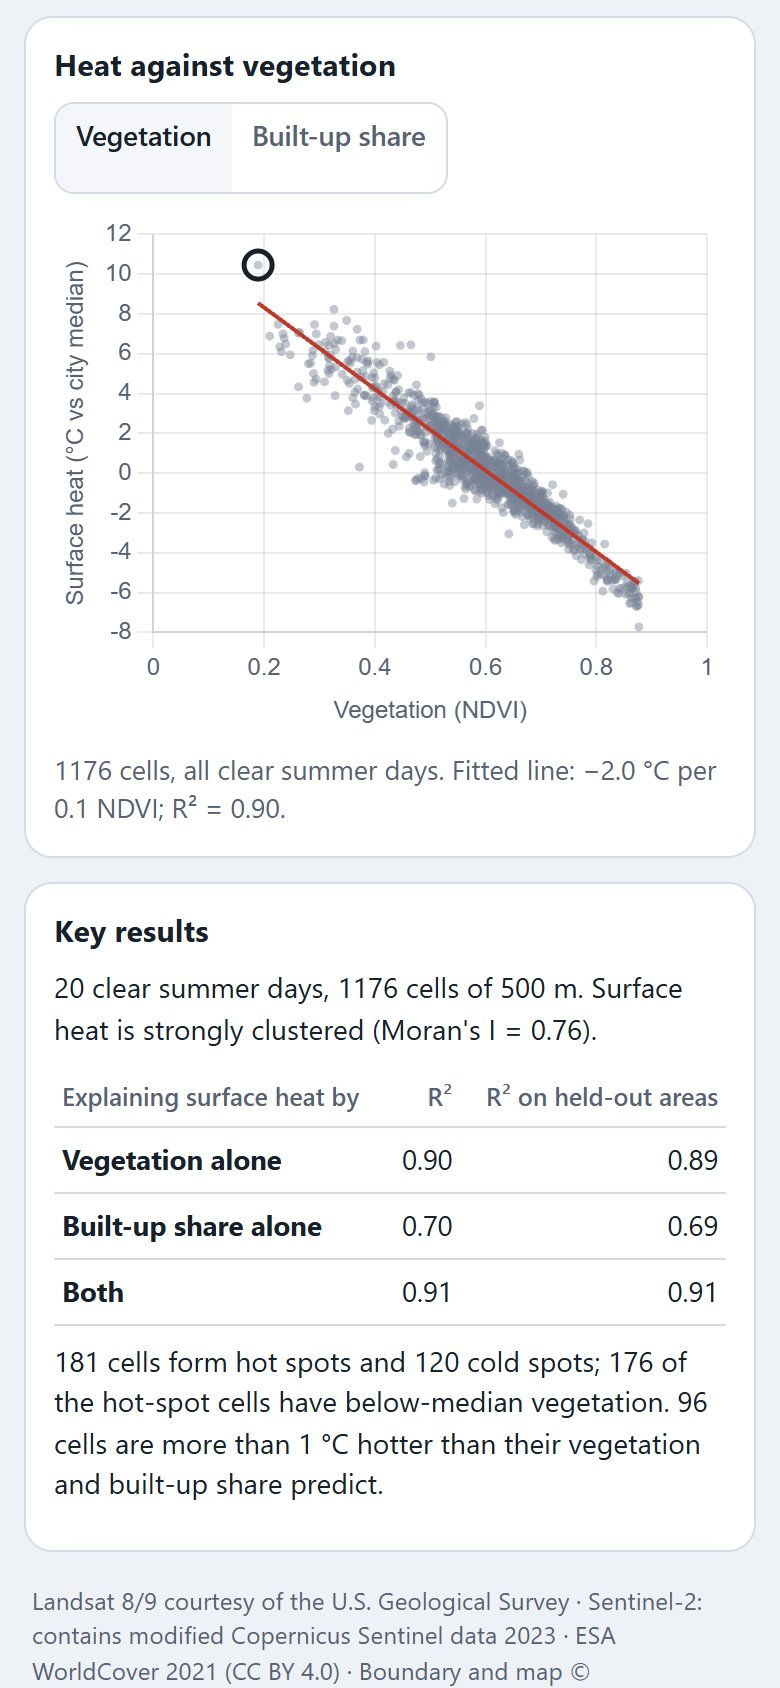
\includegraphics[width=\linewidth]{phone-chart.jpg}\caption{Scatter plot}\end{subfigure}
\caption{Phone layout (390\,px wide).}
\label{fig:phone}
\end{figure}

%======================================================================
\section{Discussion}

\paragraph{Vegetation as the main correlate.} On clear summer mornings, where Łódź is green it is cool and where it is not it is hot: vegetation explains about nine-tenths of the spatial pattern of surface heat at 500~m, on most single days and in areas the model has not seen. Built-up share explains less and adds little, because at this scale vegetation and sealing are nearly complementary. NDVI should therefore be read as a summary of land cover rather than a pure measure of greenery: a cell with low NDVI is usually also sealed. Measuring vegetation and temperature on the same day matters; it removes seasonal differences in greenness and gives an unambiguous pairing.

\paragraph{What remains.} The residual tenth is not noise. It is spatially organised and interpretable: the historic core, with its shade and street canyons, is cooler than its lack of greenery suggests; airfields and large flat-roofed industrial and commercial sites are hotter. For planning, this separates two kinds of hot place. In most hot spots, which are nearly all low in vegetation, adding greenery addresses the cause. In hotter-than-expected places, roofs and paved surfaces add heat beyond what low vegetation explains, so cool roofs, permeable paving or shading are likely to matter as much as planting.

\paragraph{Surface versus air temperature.} LST at about 11:35 local time measures surfaces in the sun, not the air at street level and not the night-time heat that matters most for health. Dense centres with shaded streets may feel different from what their surfaces suggest, and their night-time heat island can be stronger than the daytime surface one. The maps show where surfaces heat most, which is a necessary but not a sufficient guide to where people are exposed.

%======================================================================
\section{Limitations}

\begin{itemize}[leftmargin=1.2em]
  \item \textbf{Daytime surfaces only.} Landsat observes around 11:35 local time; no night-time or air-temperature data were used, and no ground measurements were available for validation.
  \item \textbf{Clear days only.} Twenty days with at least 90\% clear sky over eight summers; cloudy and humid hot days are not represented.
  \item \textbf{Associations, not effects.} The regressions describe the spatial pattern; they do not show how much planting a particular cell would cool it.
  \item \textbf{Land cover is static.} WorldCover describes 2021; land use changed in parts of the city over 2018--2025.
  \item \textbf{Gap-filled temperatures.} In 3.5\% of the city the temperature was recomputed with an estimated emissivity (error about 0.55~K); results without these cells are the same.
  \item \textbf{One city.} The strength of the vegetation–heat relationship depends on climate, urban form and scale; other cities may differ.
\end{itemize}

%======================================================================
\section{Conclusion}

On twenty clear summer days between 2018 and 2025, surface heat in Łódź was strongly clustered and closely tied to vegetation: greenery measured on the same day explains about 90\% of where the city is hotter or cooler at 500~m, robustly across days, cell sizes, edge effects and data sources. Built-up share explains less and adds little once vegetation is known. The remaining variation is spatially organised, separating places where heat follows from missing greenery from places --- such as the airport and large industrial sites --- that are hotter than greenery alone predicts, and showing a historic centre that is cooler than expected. The open pipeline and web map make each of these numbers reproducible and explorable cell by cell.

\section*{Data and code availability}

\begin{itemize}[leftmargin=1.2em]
  \item Source code, pipeline, tests, derived data and this paper: \url{\repourl}\archivedoi
  \item Web map: \url{\appurl}
  \item Rebuild everything from the satellite archives with the four scripts in the \texttt{pipeline} folder: download, analysis, web export and figures.
  \item Data sources: Landsat 8/9 courtesy of the U.S.\ Geological Survey; contains modified Copernicus Sentinel data (2023); ESA WorldCover 2021 (CC BY 4.0); boundary © OpenStreetMap contributors (ODbL).
\end{itemize}

%======================================================================
\begin{thebibliography}{99}
\small

\bibitem{benjamini1995} Y.~Benjamini and Y.~Hochberg, ``Controlling the false discovery rate: A practical and powerful approach to multiple testing,'' \emph{Journal of the Royal Statistical Society: Series B}, vol.~57, no.~1, pp.~289--300, 1995.

\bibitem{drusch2012} M.~Drusch et al., ``Sentinel-2: ESA's optical high-resolution mission for GMES operational services,'' \emph{Remote Sensing of Environment}, vol.~120, pp.~25--36, 2012.

\bibitem{hulley2015} G.~C. Hulley, S.~J. Hook, E.~Abbott, N.~Malakar, T.~Islam, and M.~Abrams, ``The ASTER Global Emissivity Dataset (ASTER GED): Mapping Earth's emissivity at 100 meter spatial scale,'' \emph{Geophysical Research Letters}, vol.~42, no.~19, pp.~7966--7976, 2015.

\bibitem{malakar2018} N.~K. Malakar, G.~C. Hulley, S.~J. Hook, K.~Laraby, M.~Cook, and J.~R. Schott, ``An operational land surface temperature product for Landsat thermal data: Methodology and validation,'' \emph{IEEE Transactions on Geoscience and Remote Sensing}, vol.~56, no.~10, pp.~5717--5735, 2018.

\bibitem{moran1950} P.~A.~P. Moran, ``Notes on continuous stochastic phenomena,'' \emph{Biometrika}, vol.~37, no.~1/2, pp.~17--23, 1950.

\bibitem{oke1982} T.~R. Oke, ``The energetic basis of the urban heat island,'' \emph{Quarterly Journal of the Royal Meteorological Society}, vol.~108, no.~455, pp.~1--24, 1982.

\bibitem{openshaw1984} S.~Openshaw, \emph{The Modifiable Areal Unit Problem}, Concepts and Techniques in Modern Geography 38. Norwich: Geo Books, 1984.

\bibitem{ord1995} J.~K. Ord and A.~Getis, ``Local spatial autocorrelation statistics: Distributional issues and an application,'' \emph{Geographical Analysis}, vol.~27, no.~4, pp.~286--306, 1995.

\bibitem{osm} OpenStreetMap contributors, ``OpenStreetMap,'' \url{https://www.openstreetmap.org}, relation 2413295, accessed 2026.

\bibitem{peng2012} S.~Peng et al., ``Surface urban heat island across 419 global big cities,'' \emph{Environmental Science \& Technology}, vol.~46, no.~2, pp.~696--703, 2012.

\bibitem{planetary} Microsoft Open Source, M.~McFarland, R.~Emanuele, D.~Morris, and T.~Augspurger, ``microsoft/PlanetaryComputer: October 2022,'' Zenodo, 2022. doi:10.5281/zenodo.7261897.

\bibitem{roberts2017} D.~R. Roberts et al., ``Cross-validation strategies for data with temporal, spatial, hierarchical, or phylogenetic structure,'' \emph{Ecography}, vol.~40, no.~8, pp.~913--929, 2017.

\bibitem{rouse1974} J.~W. Rouse, R.~H. Haas, J.~A. Schell, and D.~W. Deering, ``Monitoring vegetation systems in the Great Plains with ERTS,'' in \emph{Proceedings of the Third Earth Resources Technology Satellite-1 Symposium}, vol.~1, pp.~309--317. NASA, 1974.

\bibitem{sobrino2004} J.~A. Sobrino, J.~C. Jiménez-Muñoz, and L.~Paolini, ``Land surface temperature retrieval from LANDSAT TM 5,'' \emph{Remote Sensing of Environment}, vol.~90, no.~4, pp.~434--440, 2004.

\bibitem{voogt2003} J.~A. Voogt and T.~R. Oke, ``Thermal remote sensing of urban climates,'' \emph{Remote Sensing of Environment}, vol.~86, no.~3, pp.~370--384, 2003.

\bibitem{weng2004} Q.~Weng, D.~Lu, and J.~Schubring, ``Estimation of land surface temperature–vegetation abundance relationship for urban heat island studies,'' \emph{Remote Sensing of Environment}, vol.~89, no.~4, pp.~467--483, 2004.

\bibitem{zanaga2022} D.~Zanaga et al., ``ESA WorldCover 10 m 2021 v200,'' Zenodo, 2022. doi:10.5281/zenodo.7254221.

\bibitem{zhou2011} W.~Zhou, G.~Huang, and M.~L. Cadenasso, ``Does spatial configuration matter? Understanding the effects of land cover pattern on land surface temperature in urban landscapes,'' \emph{Landscape and Urban Planning}, vol.~102, no.~1, pp.~54--63, 2011.

\end{thebibliography}

\end{document}
